% Chapter Template

\chapter{Search Algorithms} % Main chapter title

\label{Chapter4} % Change X to a consecutive number; for referencing this chapter elsewhere, use \ref{ChapterX}

In this chapter, the search algorithms used for this project are explained in more detail and how they have been adapted for this particular application.\\\\
These two search algorithms are used to find a target value in a sorted list of values. For this project, what we are trying to find is the minimum value for the cost function, and the list of values are all the integers between the minimum and the maximum possible values for the cost function.

\begin{center}
	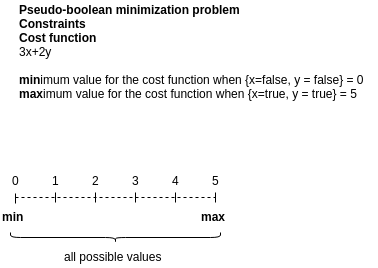
\includegraphics[width=0.8\textwidth]{Figures/Search_space.png}
	\captionof{figure}{Search Space}
	\label{search_space}
\end{center}
As the reader can see from the figure above, the search problem we are facing can be described as one where the search space is formed by integers between \emph{min} and \emph{max} and our target value is unknown.

\paragraph{How can we know that a value is the minimum, i.e. our target?\\}
If $m$ is the minimum value, we know that the constraint formed by $cost function \leq m$ is satisfiable whereas the constraint $cost function \leq m-1$ is unsatisfiable.\\
\begin{center}
	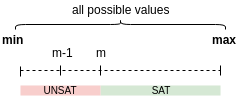
\includegraphics[width=0.8\textwidth]{Figures/SearchSpace2.png}
	\captionof{figure}{Satisfiability of the search space given a minimum value}
	\label{search_space_2}
\end{center}
This is the property used to check if the value found is minimum or not.

\section{Linear search}

Linear search is an algorithm which sequentially checks all the values for the target value until it is found or all the elements have been visited.\\
The search can start with the smallest value or the biggest one. For this application, the initial value is \emph{max} and the algorithm traverse the search space descending until \emph{min}.\\
This decision was made because proving satisfiability of a problem is easier (faster) than proving it is unsatisfiable. Also, given $m$ and $n$ where $n < m$, if $cost function \leq m$ is unsatisfiable then $cost function \leq n$ will also be unsatisfiable. \\
As previously said, the algorithm starts with \emph{max}, which means that it generates the Pseudo-Boolean constraint $cost function \leq max$. If the problem is unsatisfiable with this value, it can be deduced that with other values will also be unsatisfiable and therefore the search can end.\\
Otherwise, it keeps this value as the possible minimum and tries the next one until it finds an unsatisfiable one or the \emph{min}, which is the last value to be checked.\\
Once the algorithm finished, the last found possible value becomes the minimum, or if no possible minimum was found, the problem is unsatisfiable.\\\\
The class \emph{LinearSearchStrategy}\footnote{\href{https://github.com/marcbenedi/SAT-tfg/blob/master/source_files/LinearSearchStrategy.cpp}{Source code in Github}} implements this algorithm. Let's explain its essential parts:\\\\
Firstly, the following variables are initialised:
\begin{verbatim}
int64_t min_costFunc = pm.getCostFunctionMin();
int64_t k = pm.getCostFunctionMax();
min = pm.getCostFunctionMax()+1;
\end{verbatim}
\begin{itemize}
	\item \emph{min\_costFunc} is used to limit the last value to look at
	\item \emph{k} is the value it checks. As previously said, initially is the maximum possible value for the cost function
	\item \emph{min} is the last minimum value found. Initialised with an invalid value which is the maximum plus one
\end{itemize}
Then the first constraint is created. The algorithm takes advantage of the \emph{Incremental Constraints} functionality of PBLib.
\begin{verbatim}
IncPBConstraint inc_costFunction = IncPBConstraint(w_costFunction, PBLib::LEQ, k);
pb2cnf.encodeIncInital(inc_costFunction, cdb, auxVarManager);
\end{verbatim}
It creates an incremental constraint with the $cost function \leq k$ and then encodes it into a CNF.\\\\
The next part is the loop, the linear search implementation:
\begin{verbatim}
bool end = false;
while (!end) {
    if (k == min_costFunc) {
        end = true;
    }
	
    inc_costFunction.encodeNewLeq(k, cdb, auxVarManager);
	
    bool t_sat;
    (solver->*solve)(temp_model, cdb.getClauses(),t_sat);
	
    if (t_sat) {
        model = temp_model;
        min = k;
        k--;
    }
    else{
        end = true;
    }
}
\end{verbatim}
The loop can end for two reasons:
\begin{itemize}
	\item \emph{k == min\_costFunc}: this is the last value to check
	\item \emph{t\_sat is false}: the current iteration is unsatisfiable, i.e. the next values in the search space will also be unsatisfiable 
\end{itemize}
After encoding the new constraint $cost function \leq k$, it calls the solver.\\\\
If it is \emph{satisfiable}, the model is stored and $k$ is stored as the las $min$ found.\\
If after ending the search no other minimum has been found, that is returned along with its model. After that, a new iteration is done with $k=k-1$.

\section{Binary search}
Binary search is an algorithm which looks for a value in a given sorted input.\\
As before, our inputs is the integers between \emph{min} and \emph{max}, and therefore they are sorted.\\
In the beginning, Binary search takes the middle value and compares it with the target value. If it is bigger than the target, then it looks for the value in the subspace between minimum value and the value before the middle one. If it is smaller than the target, then it looks for the value in the subspace between the value after the middle one and the maximum.\\
For this application, the leftmost value of the search is \emph{min}, and the rightmost value for the search is \emph{max}. Again, our target value is the minimum one. For each iteration, the algorithm checks that the left side of the problem is less or equal than the right side because otherwise, the state of the search would be incorrect. \\
If this is true, then it gets the middle value between them and generates the constraint $cost function \leq middle value$, which is added with the other constraints and then encoded into a CNF. If the CNF is satisfiable, then the middle value is stored as a possible minimum, and the search continues with a new space contained between the left side and the integer between the middle value. Otherwise, if the CNF is unsatisfiable, it checks if the stored possible minimum is exactly the integer after the middle value because then the integer would be the minimum value.\\
If not, it continues the search with a new space contained between the integer after the middle value and the right side.\\\\
The class \emph{BinarySearchStrategy}\footnote{\href{https://github.com/marcbenedi/SAT-tfg/blob/master/source_files/BinarySearchStrategy.cpp}{Source code in Github}} implements this algorithm:\\\\
As previously said, the search space is limited between \emph{min} and \emph{max}. For this reason, the variables \emph{left} and \emph{right} are initialised as following:
\begin{verbatim}
left = p.getCostFunctionMin();
right = p.getCostFunctionMax();
\end{verbatim}
As in \emph{LinearSearchStrategy}, the value \emph{min} is initialised as the maximum value for the cost function plus one.
\begin{verbatim}
min = right + 1;
\end{verbatim}
Let's now explain the loop which implements the binary search algorithm:
\begin{verbatim}
while (not end) {
    if(left<=right){
        cnf.clear();
        cnf.insert(cnf.end(),cnf_constraints.begin(),cnf_constraints.end());
    
        int64_t k = (left+right)/2;
    
        if (left == right) {
            //no more values to try
            end = true;
        }
    
        firstFreshVariable = pb2cnf.encodeLeq(pm.getCostFunction().getWeights(), pm.getCostFunction().getLiterals(), k, cnf, firstFreshVariable) + 1;
    
        bool t_sat;
        (solver->*solve)(temp_model, cnf,t_sat);
    
        if (t_sat) {
            min = k;
            right = k-1;
            model = temp_model;
        }
        else{
            if (min == k + 1) {
                end = true;
            }
            left = k+1;
        }
    }
    else{
        end = true;
    }
}
\end{verbatim}
The search can end for three reasons:
\begin{itemize}
	\item \emph{left==right}: it is checking the last value, therefore there are no values left for the next iterations
	\item \emph{k unsatisfiable but k+1 satisfiable}: then \emph{k+1} is the minimum and the search finishes
	\item \emph{left > right}: the state of the search is inconsistent because it has checked all the values of the space
\end{itemize}
The first thing it does is clean the CNF and inserting the constraints of the problem again. Then, it calculates the next value to check, which is the one in the middle, and generates the constraint $cost function \leq k$. Finally, the CNF is passed to the solver.\\\\
If the CNF is \emph{satisfiable}, then \emph{k} is stored as the las minimum seen along with its model. The right side of the space is limited to \emph{k-1}.\\
Otherwise, the left side of the space is limited to \emph{k+1}, and as previously said, it checks if the last minimum value found equals \emph{k+1}.